% +------------------------------------------------------------------------------------------------------------------+
%  (20 баллов) Дан массив, содержащий перестановку чисел от 0 до N. Вычислить ожидаемое 
%  число поворотов каждого типа при добавлении этого массива в пустое 
%  авл дерево(провести численный эксперимент)
% +------------------------------------------------------------------------------------------------------------------+

\documentclass[a4paper,12pt] {report} 			% размер бумаги устанавливаем А4, шрифт 12пунктов
\usepackage[utf8] {inputenc} 					% включаем свою кодировку: utf8
\usepackage{graphicx}						% подключаем графический модуль
\graphicspath{{pictures/}}						% путь к картинкам
\usepackage[english,russian] {babel} 			% используем русский и английский языки с переносами
\usepackage{misccorr}						% соответствие стандарту
\usepackage{listingsutf8}

\begin{document}

\setlength{\parskip}{4pt}

\begin{center}
	{\LARGE \bfseries \slshape Анализ количества поворотов при добавлении перестановки из N элементов в АВЛ дерево}
\end{center}

\textit
{
	Дан массив, содержащий перестановку чисел от 0 до N. Найти среднее кол-во поворотов каждого типа. Провести численный эксперимент.
}

\section{Введение в теорию}

{\bfseries Двоичное дерево поиска} -- это двоичное дерево, для которого выполняются следующие дополнительные условия: У всех узлов левого 
поддерева произвольного узла значения ключей данных меньше, нежели значение ключа данных самого этого узла; У всех узлов правого 
поддерева произвольного узла значения ключей данных больше либо равны, нежели значение ключа данных самого этого узла.

{\bfseries Сбалансированное дерево} -- дерево, высота которого логарифмична кол-ву элементов.

{\bfseries АВЛ дерево} -- это бинарное дерево поиска, в котором для каждого элемента выполнено свойство: разница высот для
левого и правого поддерева по модулю не превосходит $1$. Данное условие является достаточным для сбалансированности дерева.

При стандартной вставке элементов в дерево поиска оно перестает быть сбалансированным. Для предотвращения этого
используются следующие методы:

\begin{enumerate}
	\item {\bfseries Малый левый поворот}
	\item {\bfseries Большой левый поворот}
	\item {\bfseries Малый правый поворот}
	\item {\bfseries Большой правый поворот}
\end{enumerate}

{\bfseries Повороты дерева} - это операции, которые позволяют изменить структуру дерева не меняя порядка элементов. Используя их для 
соответствующих узлов, можно минимизировать высоту дерева, то есть сделать его сбалансированным.

% <<<<малые повороты>>>>
\begin{figure} [h]
\center{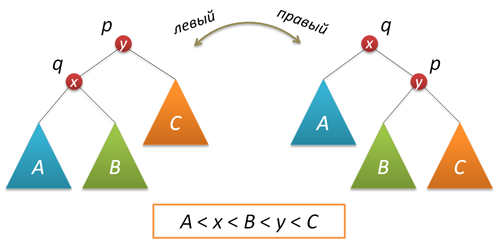
\includegraphics [scale = 0.6] {picture1.png}}
\caption{Малые повороты. Разность высот поддеревьев по модулю равна 2, производим следующую трансформацию дерева}
\end{figure}
% <<<<малые повороты>>>>

% <<<<большие повороты>>>>
\begin{figure} [h]
\center{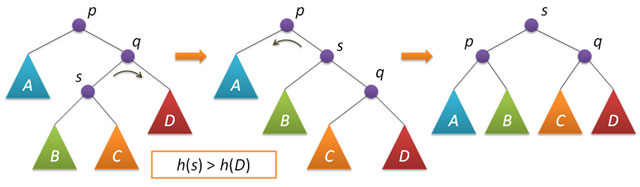
\includegraphics [scale = 0.6] {picture2.png}}
\caption{Большой поворот применяется при условии $h(s)>h(D)$ и сводится в данном случае к двум 
простым -- сначала правый поворот вокруг q и затем левый вокруг p}
\end{figure}
% <<<<большие повороты>>>>

\section{Эксперимент}

Для проведения эксперимента была написана программа на языке С++ (файлы программы расположены в папке \textbf{programm\_14} там же расположен
тестовый файл \textbf{stdout.txt}, в котором расположен стандартный вывод программы). 
Она генерирует случайную перестановку из $N$ элементов, записывает ее в АВЛ дерево поэлементно, при необходимости применяя повороты. При этом 
происходит подсчет их количества. Эта процедура повторяется несколько раз, после чего все значения усредняются.

Чтобы выявить зависимости эксперимент проводился для различных значений $N$, а именно для $N \in {500, 600, 700, \ldots, 2000}$.
Главным образом это все было предназначено для анализа пропорциональности роста кол-ва поворотов различного типа в зависимости от числа $N$.

\section{Результаты и выводы}

Вывод программы перенаправлялся в файл \textbf{output.txt} в папке \textbf{documents}. По полученным результатам был построен график зависимости кол-ва 
различных поворотов от числа  $N$. Эксперимент показал, что зависимость кол-ва поворотов каждого типа, от количества элементов перестановки с некоторой 
погрешностью линейна.

% <<<<график зависимости>>>>
\begin{figure} [h]
\center{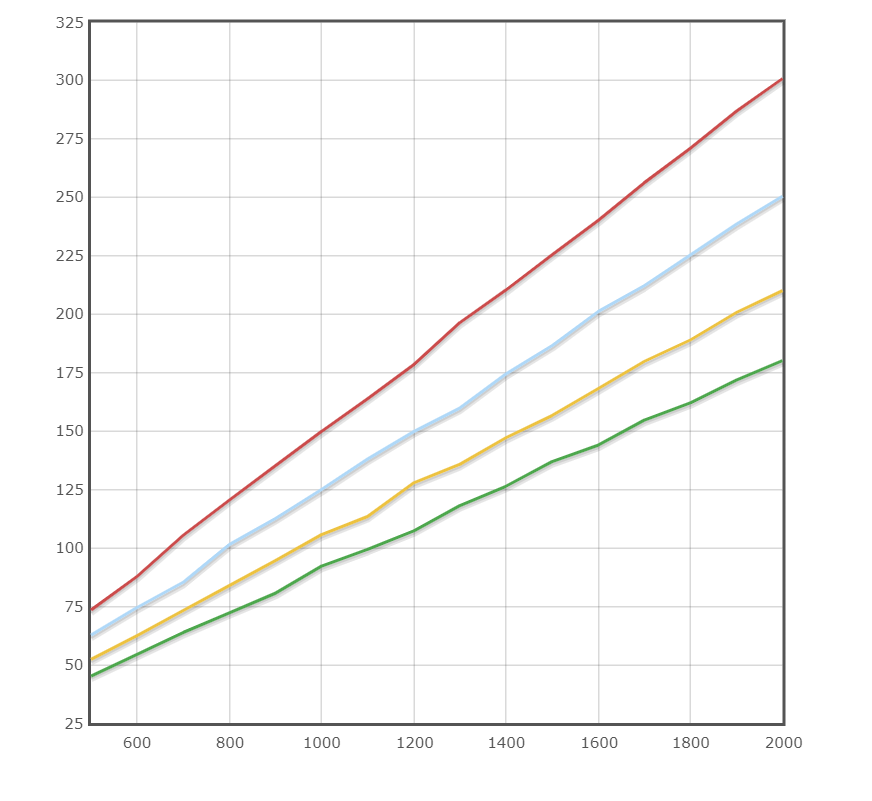
\includegraphics [scale = 0.5] {graph.png}}
\caption{Малый левый поворот -- красная линия; Большой правый поворот -- голубая линия; Большой левый поворот -- желтая линия; 
Малый правый поворот -- зеленая линия.}
\end{figure}
% <<<<график зависимости>>>>

Несложно рассчитать коэффициенты пропорциональности:

\begin{enumerate}
	\item Малый левый поворот : $k \approx 0,150$
	\item Большой левый поворот : $k \approx 0,105$
	\item Малый правый поворот : $k \approx 0,090$
	\item Большой правый поворот : $k \approx 0,125$
\end{enumerate}

\end{document}
